% Appendix A

\chapter{Circuits} % Main appendix title

\label{AppendixB} % For referencing this appendix elsewhere, use \ref{AppendixA}

\lhead{Appendix B. \emph{Circuit Figures}} % This is for the header on each page - perhaps a shortened title

\begin{figure}[ht]
\centering
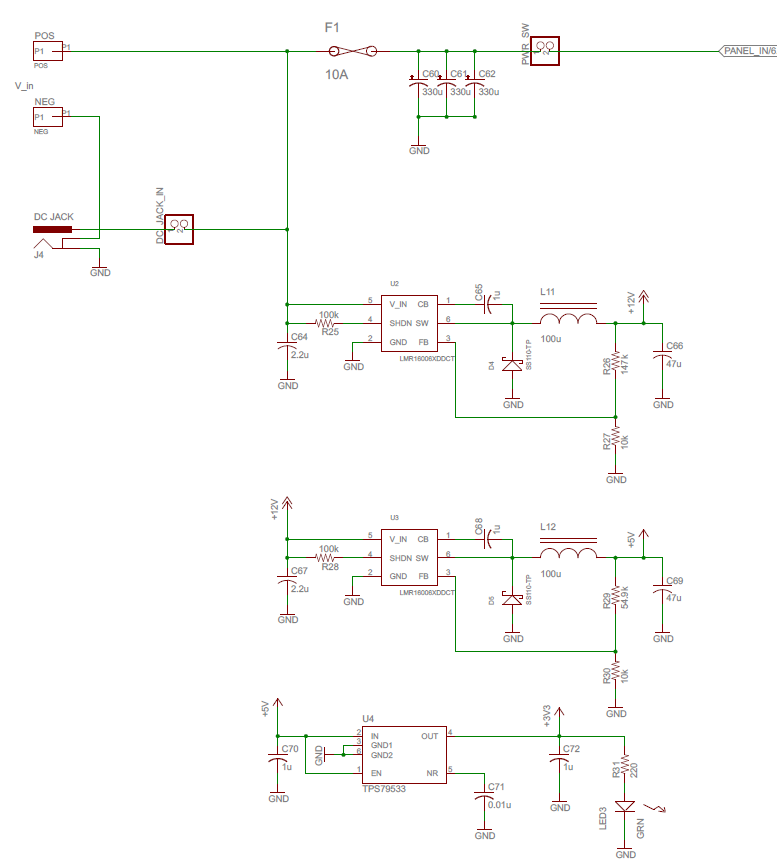
\includegraphics[width = 3.5in]{logic_power.PNG}
\caption{Logic Power Supply Circuit}
\label{logic power fig}
\end{figure}


\begin{figure}[hb]
\centering
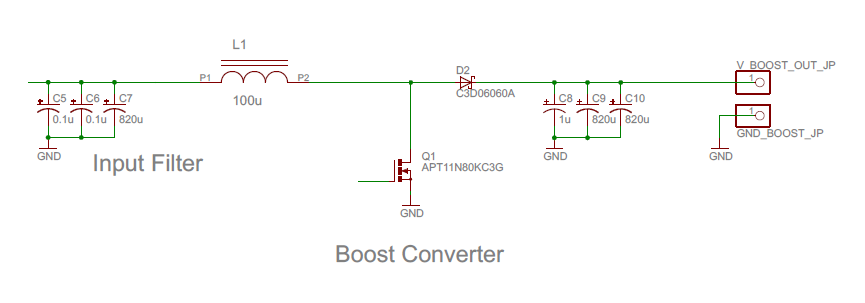
\includegraphics[width = 3.5in]{sch_boost.png}
\caption{Boost Converter Circuit}
\label{boostConverterCircuit}
\end{figure}

\begin{figure}[ht]
\centering
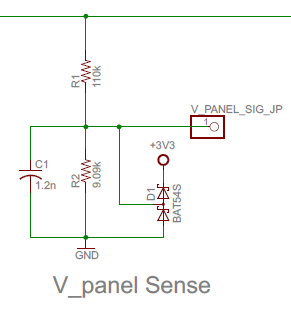
\includegraphics[width = 3.5in]{sch_Vpanel.png}
\caption{PV Voltage Sense Circuit}
\label{VpvSenseCircuit}
\end{figure}

\begin{figure}[hb]
\centering
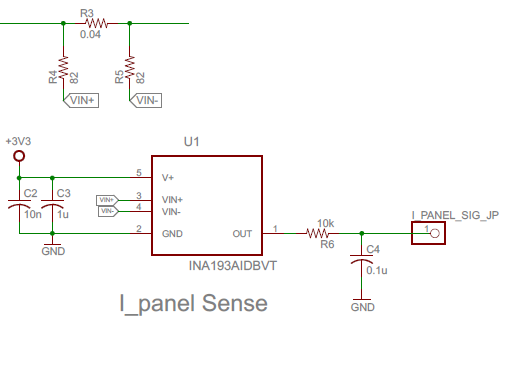
\includegraphics[width = 3.5in]{sch_Ipanel.png}
\caption{PV Current Sense Circuit}
\label{IpvSenseCircuit}
\end{figure}

\begin{figure}[ht]
\centering
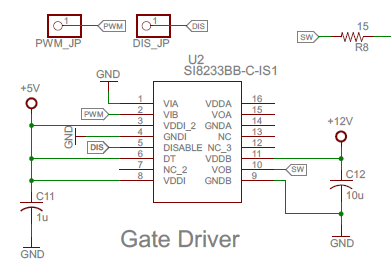
\includegraphics[width = 3.5in]{sch_driver.png}
\caption{ Gate Driver Circuit}
\label{gateDriverCircuit}
\end{figure}

\begin{figure}[hb]
\centering
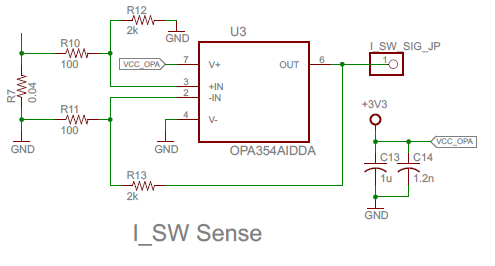
\includegraphics[width = 3.5in]{sch_Isw.png}
\caption{Switch Current Sense Circuit}
\label{IswSenseCircuit}
\end{figure}

\begin{figure}[ht]
\centering
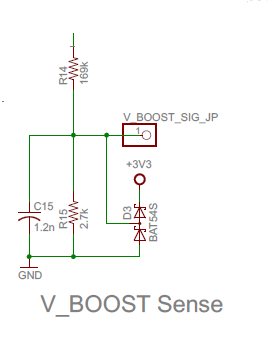
\includegraphics[width = 3.5in]{sch_Vboost.png}
\caption{Boosted Voltage Sense Circuit}
\label{VboostSenseCircuit}
\end{figure}

\begin{figure}[hb]
\centering
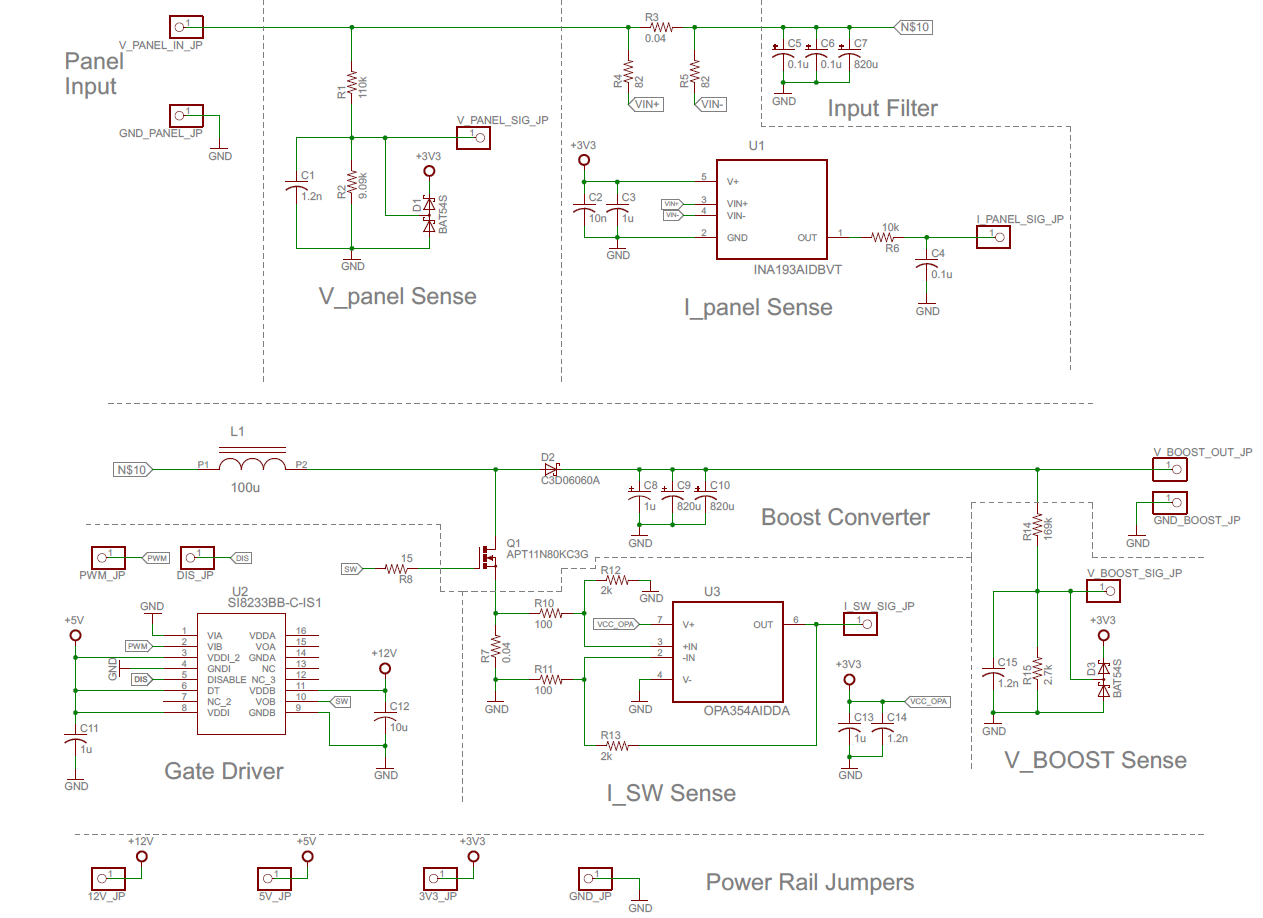
\includegraphics[width = 3.5in]{Boost_Schematic.PNG}
\caption{Boost Converter Schematic}
\label{boostCompleteSchematic}
\end{figure}

\begin{figure}[ht]
\centering
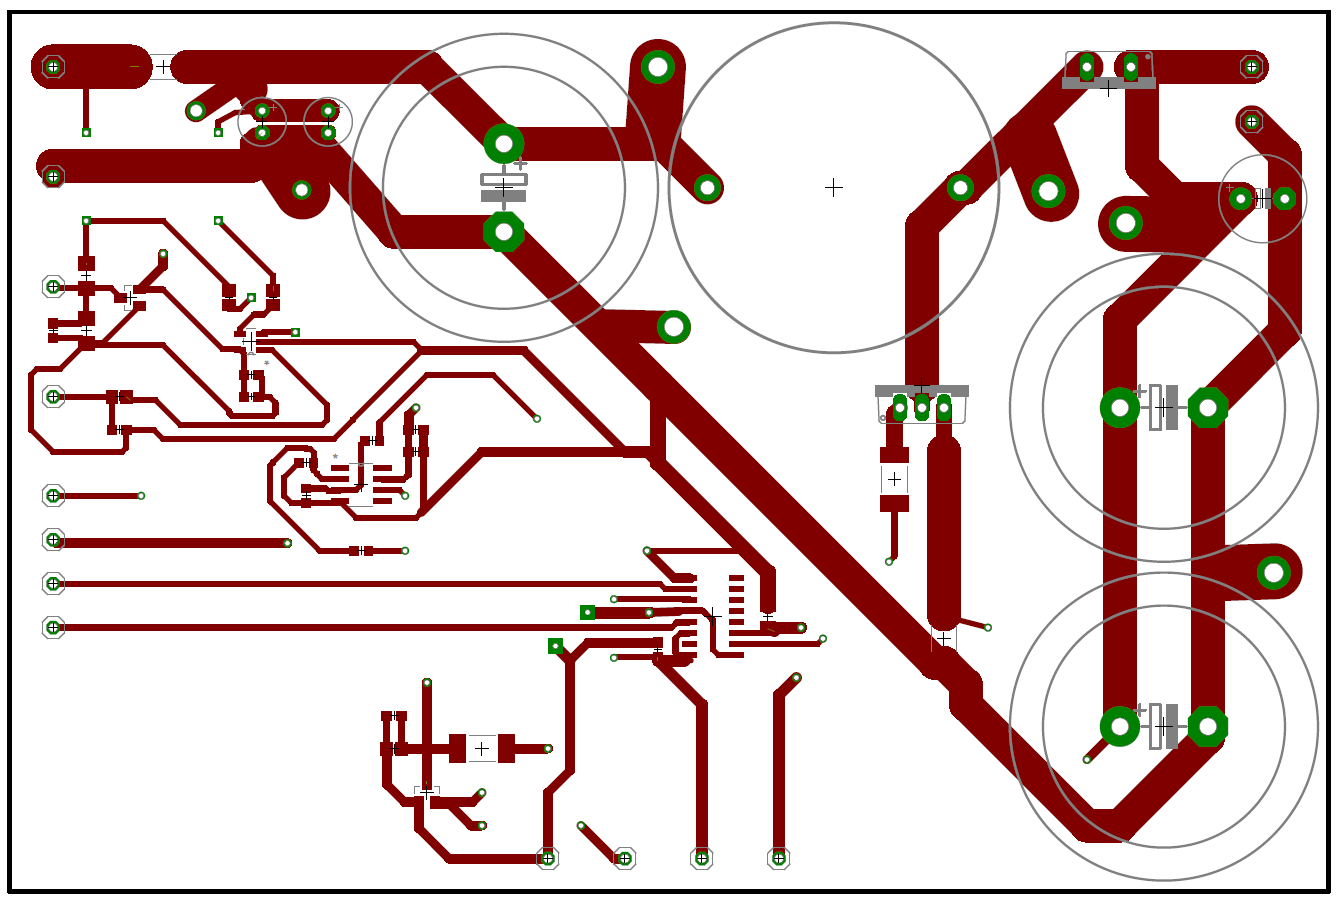
\includegraphics[width = 3.5 in]{Boost_PCB_TOP.PNG}
\caption{Boost Board PCB Top}
\label{boostPCBTop}
\end{figure}

\begin{figure}[hb]
\centering
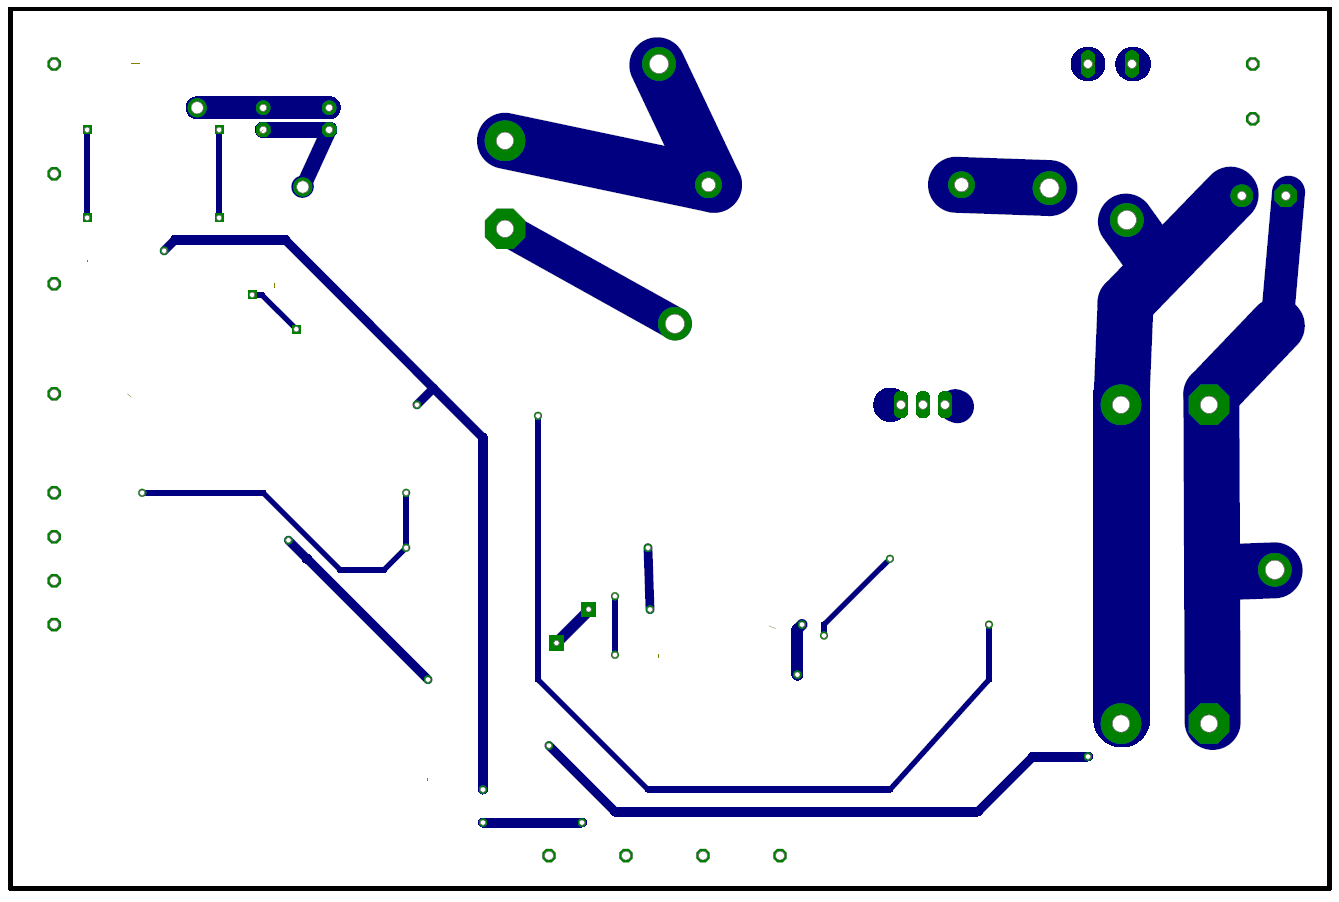
\includegraphics[width = 3.5 in]{Boost_PCB_BOTTOM.PNG}
\caption{Boost Board PCB Bottom}
\label{boostPCBBottom}
\end{figure}

\begin{figure}[ht]
\centering
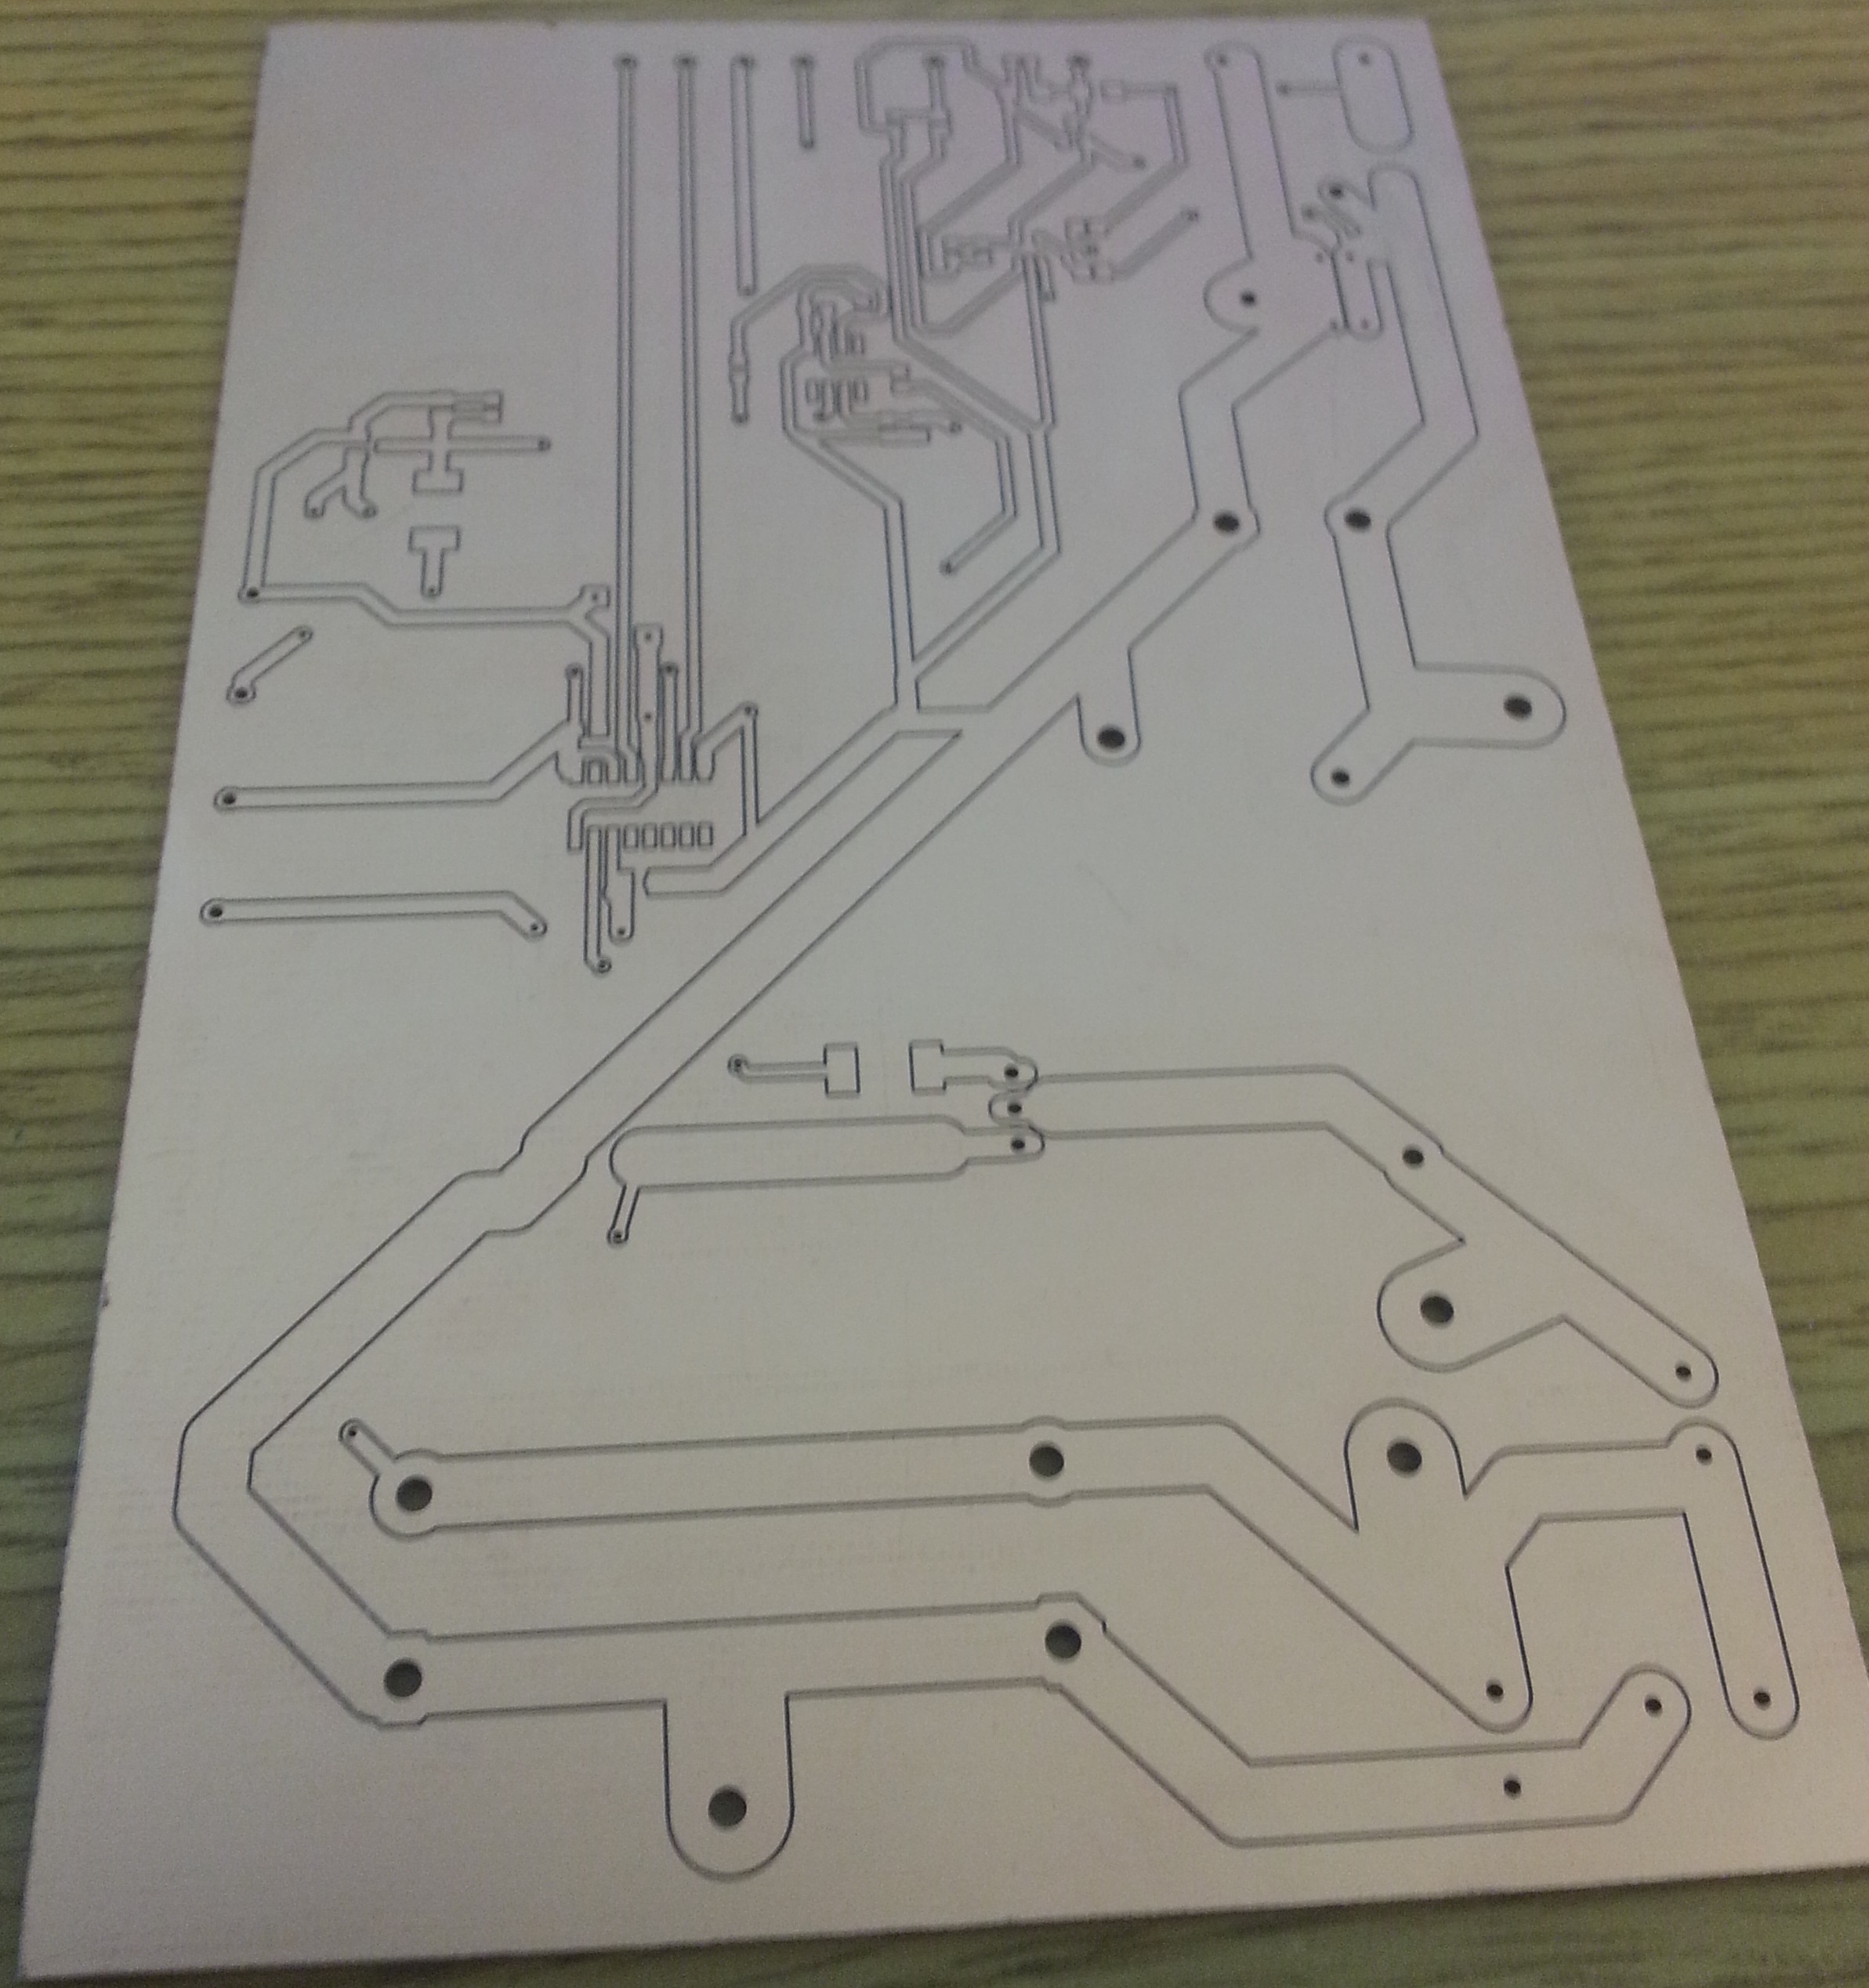
\includegraphics[width = 3.5in]{boost_PCB_routed.jpg}
\caption{Board Board PCB}
\label{unpopulatedBoostPCB}
\end{figure}

\begin{figure}[hb]
\centering
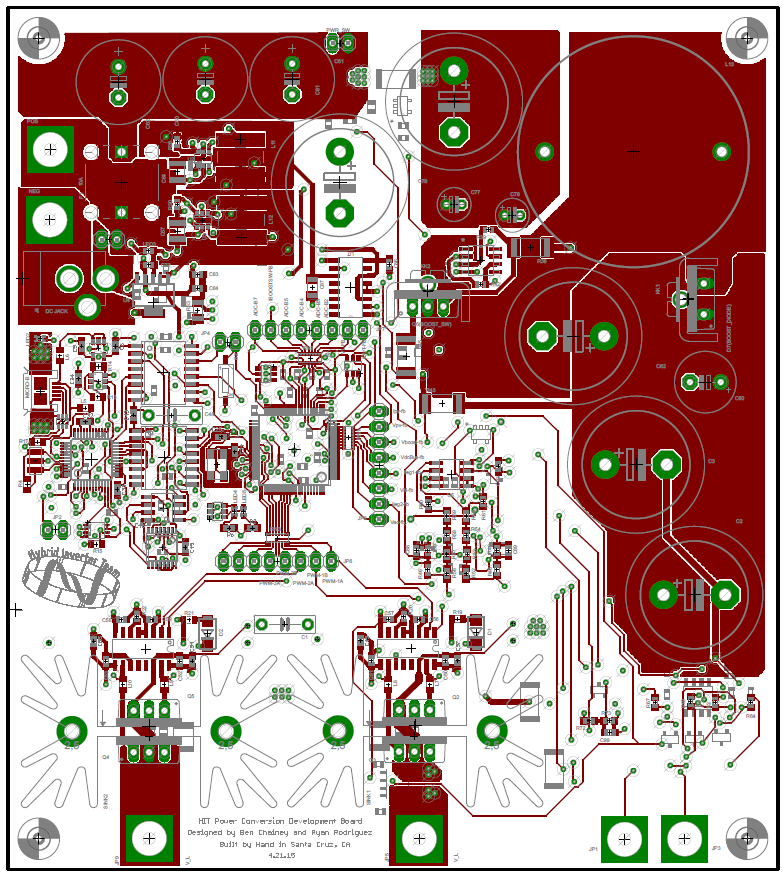
\includegraphics[width = 3.5in]{PCB_top}
\caption{Hit Board Rev 1, Top}
\label{PCB Top}
\end{figure}

\begin{figure}[ht]
\centering
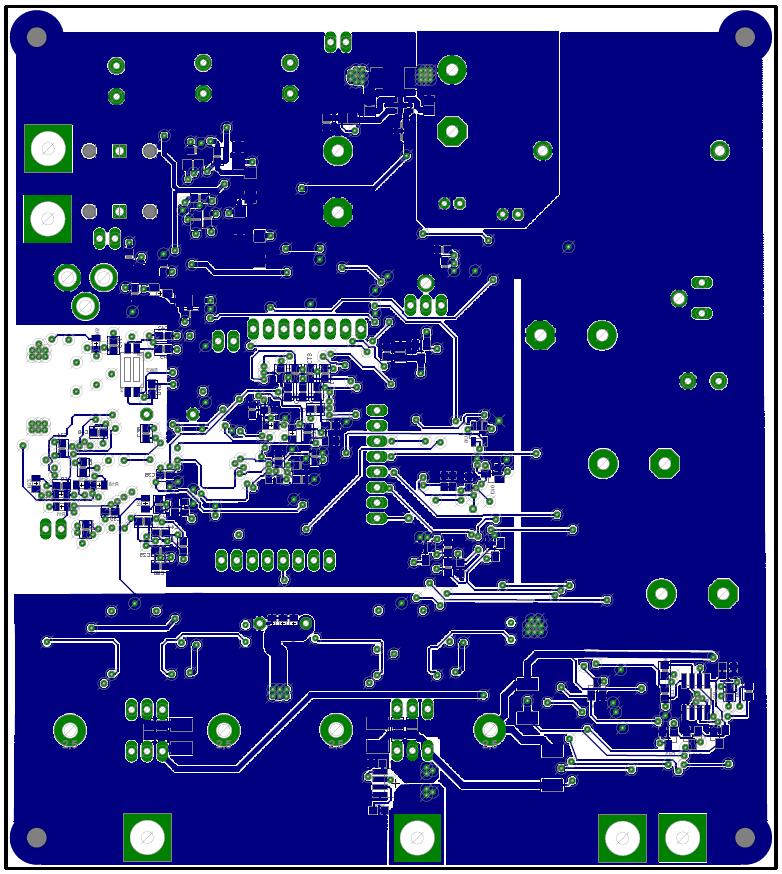
\includegraphics[width = 3.5in]{PCB_bottom}
\caption{Hit Board Rev 1, Bottom}
\label{PCB Bottom}
\end{figure}

\begin{figure}[hb]
\centering
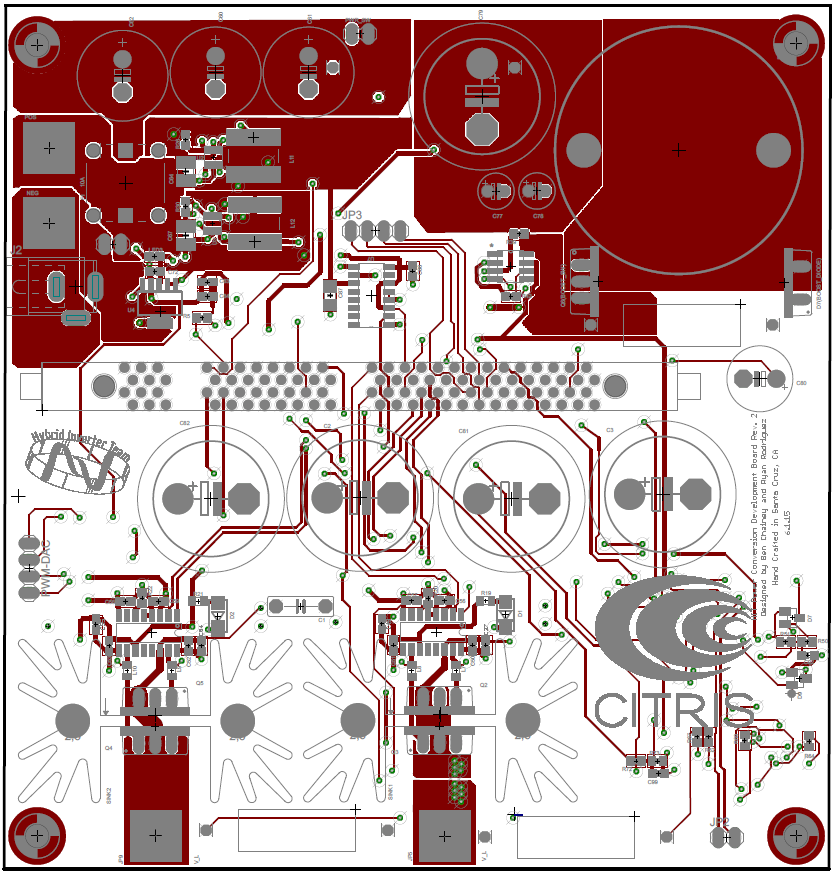
\includegraphics[width = 3.5in]{HIT_Gen2_PCB_Top}
\caption{HIT Board Gen.2 Layout Top}
\label{HIT Board Rev 2, Top}
\end{figure}

\clearpage

\begin{figure}[ht]
\centering
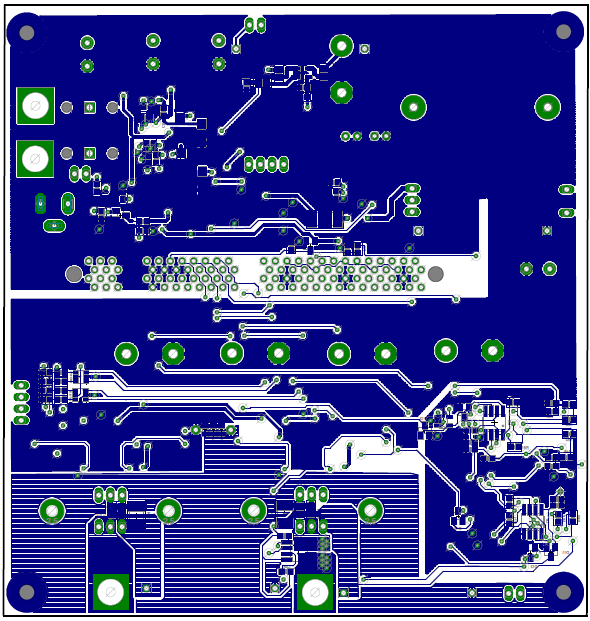
\includegraphics[width = 3.5in]{HIT_Gen2_PCB_Bottom}
\caption{HIT Board Gen.2 Layout Bottom}
\label{HIT Board Rev 2, Bottom}
\end{figure}

\begin{figure}[hb]
\centering
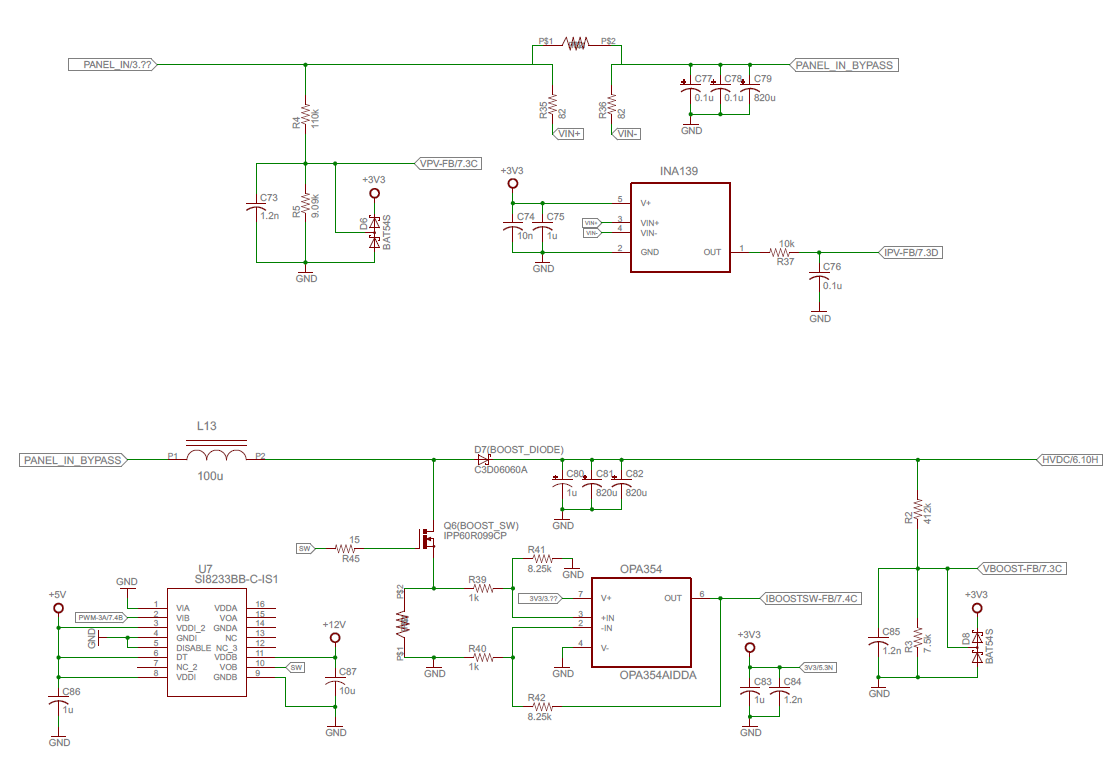
\includegraphics[width = 3.5in]{HIT_Gen2_boost_sch}
\caption{HIT Board Rev.2 Boost Schematic}
\label{Rev2 boost sch}
\end{figure}

%\begin{figure}[h]
%\centering
%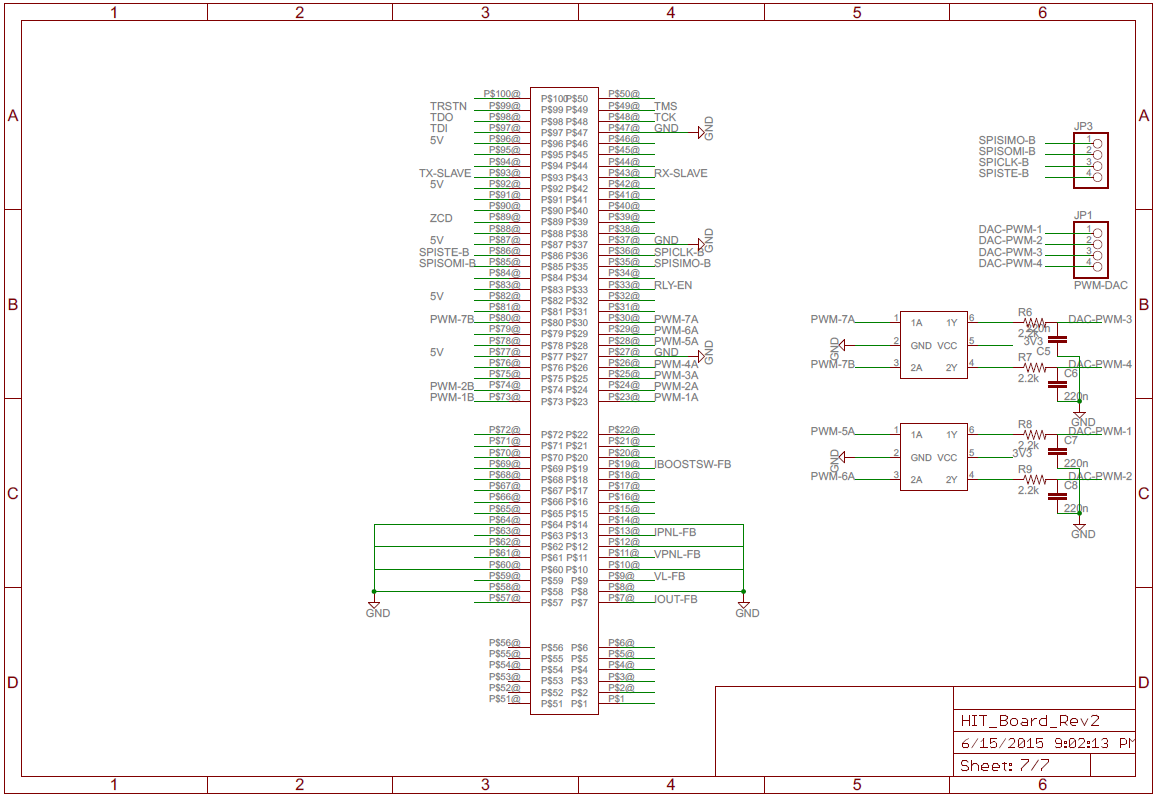
\includegraphics[width = 3.5in]{HIT_Gen2_dimm_sch.PNG}
%\caption{HIT Board Rev.2 Dimm Schematic}
%\label{Rev2 dimm sch}
%\end{figure}

\begin{figure}[ht]
\centering
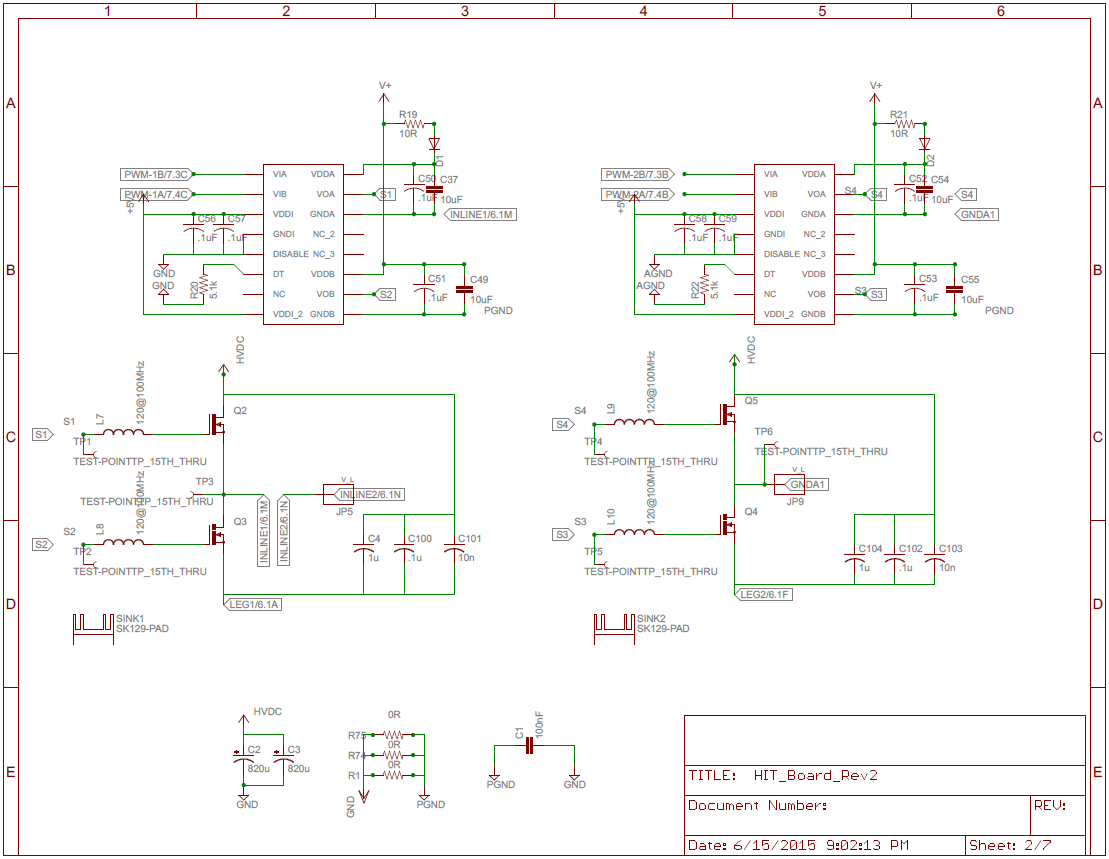
\includegraphics[width = 3.5in]{HIT_Gen2_hbridge_sch.PNG}
\caption{HIT Board Rev.2 H-Bridge Schematic}
\label{Rev2 hbridge sch}
\end{figure}

\begin{figure}[hb]
\centering
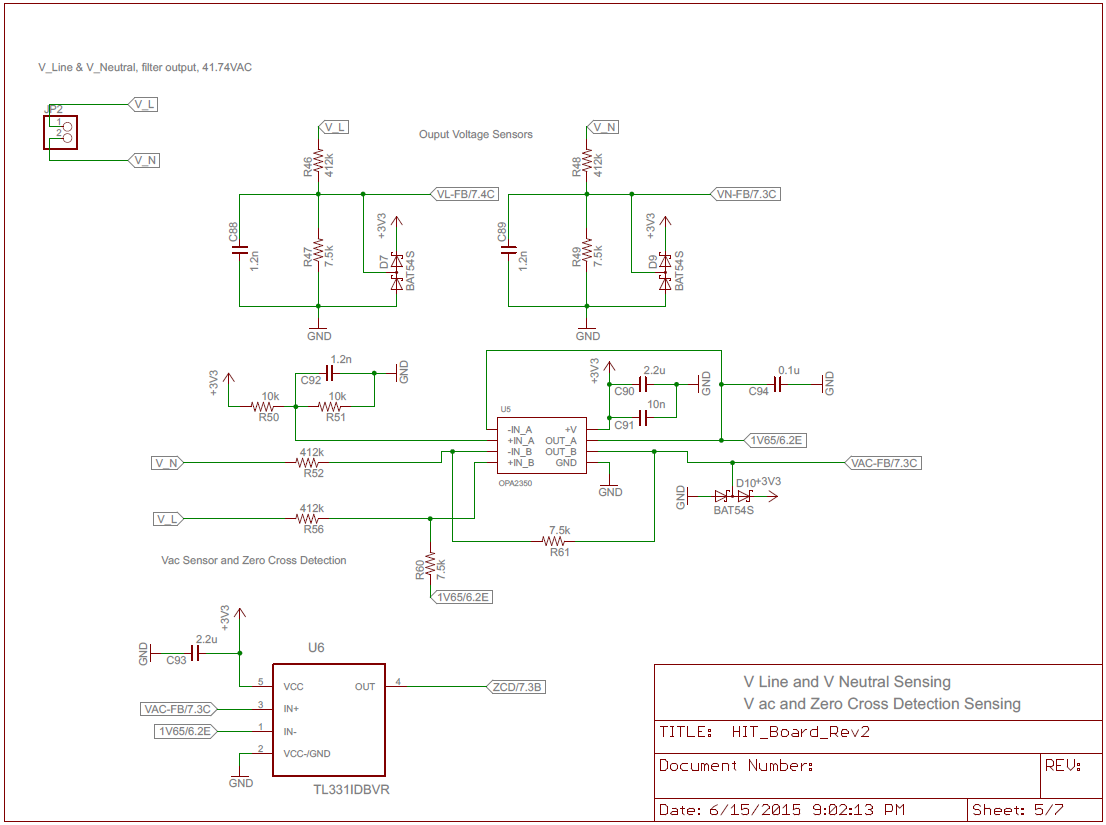
\includegraphics[width = 3.5in]{HIT_Gen2_sense1_sch.PNG}
\caption{HIT Board Rev.2 Output Sensors 1 Schematic}
\label{Rev2 sense1 sch}
\end{figure}

\begin{figure}[ht]
\centering
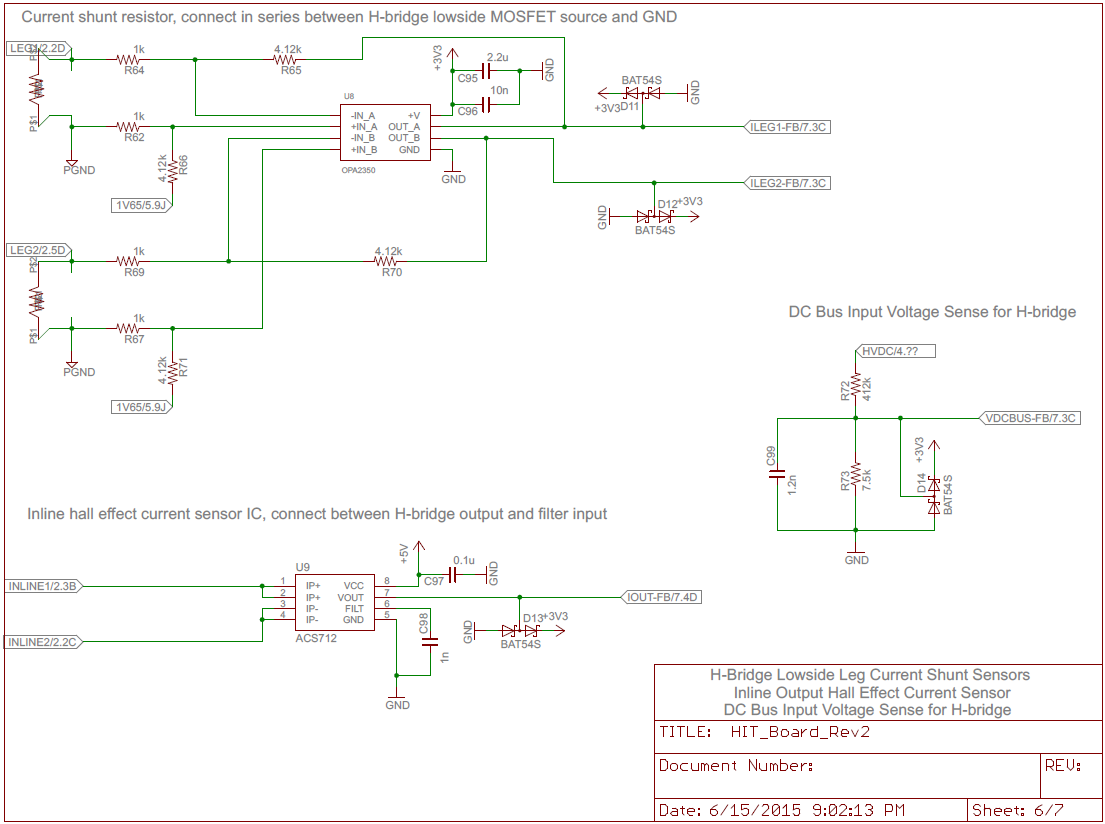
\includegraphics[width = 3.5in]{HIT_Gen2_sense2_sch.PNG}
\caption{HIT Board Rev.2 Output Sensors 2 Schematic}
\label{Rev2 sense2 sch}
\end{figure}

